\documentclass[a4paper,11pt]{article}
\usepackage[top=16mm,bottom=20mm,left=16mm,right=16mm]{geometry}
\usepackage{fontspec}
\usepackage{xeCJK}
\setmainfont{Times New Roman}
\setCJKmainfont{Yu Gothic}
\setmonofont{Consolas}
\setCJKmonofont{Yu Gothic}
\usepackage{graphicx}
\usepackage{booktabs}
\usepackage{longtable}
\usepackage{tabularx}
\usepackage{array}
\usepackage{amsmath}
\usepackage{enumitem}
\usepackage{tikz}
\usetikzlibrary{arrows.meta,calc,positioning,shapes.geometric}
\usepackage[unicode]{hyperref}
\hypersetup{
  colorlinks=true,
  linkcolor=blue,
  urlcolor=blue,
  pdftitle={Solar package all-in-one manual},
  pdfauthor={Codex}
}
\setlength{\parskip}{0.45em}
\setlength{\parindent}{1em}
\renewcommand{\arraystretch}{1.18}
\newif\ifanswers
\answerstrue
\newcommand{\fillin}[2]{\ifanswers{\textbf{#1}}\else\underline{\hspace{#2}}\fi}
\newcommand{\sourcepath}[1]{\path{#1}}
\newcommand{\cmd}[1]{\texttt{#1}}
\newcommand{\keypoint}[1]{\fbox{\parbox{0.95\linewidth}{#1}}}

\title{改良版ソーラーカーパッケージ\\オールインワン解説書兼体験ワーク}
\author{solar\_ws0129-main}
\date{2026-07-16}

\begin{document}
\maketitle

\section*{本書の目的}
本書は、現在の改良版ソーラーカーパッケージについて、
\begin{itemize}[leftmargin=1.5em]
  \item PowerShell 入口から何が起動するか
  \item offline simulation / live / live\_wifi / measure / forecast / identify がどのように繋がるか
  \item 実測ログからの MLE 同定がどの数式で行われ、どの profile / map / planner へ反映されるか
  \item WiFi 文字列テレメトリをソーラーカー側・伴走車側でどう送受信すればよいか
  \item 現在の maps / coefficients の意味と所在
\end{itemize}
を一冊で追えるようにまとめたものである。

PASSO 系列と磁力関連は本書の主対象から外し、ソーラーカー本体の planner / sim / live 運用に集中する。

\keypoint{
\textbf{重要な結論:}
現在の package の本質は PowerShell / shell の入口、launch、
\sourcepath{mpc_solarcar/*.py}、offline sim、車両同定、各 \sourcepath{profile.yaml} にある。
本書では、この入口から物理モデル、同定、運用までを一貫して説明する。
}

\tableofcontents
\newpage

\section{まず最初に全体像}
\subsection{一番上の流れ}
\begin{center}
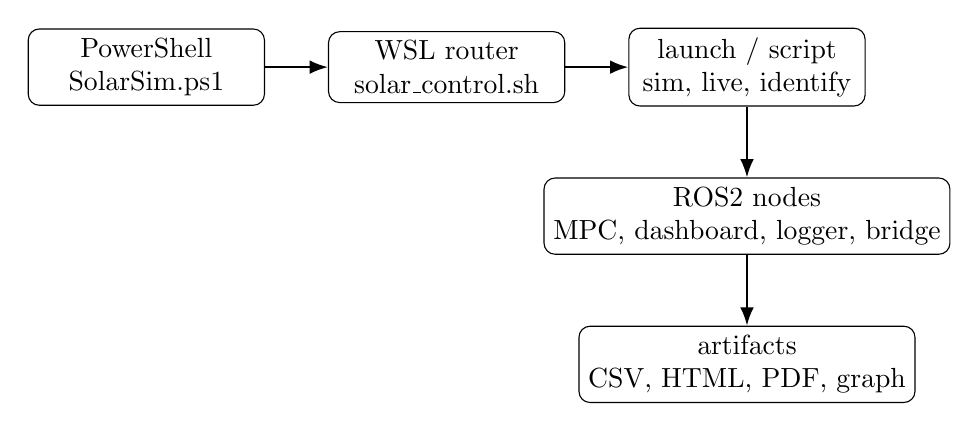
\begin{tikzpicture}[
  node distance=9mm and 8mm,
  box/.style={draw, rounded corners, align=center, minimum width=30mm, minimum height=9mm},
  arr/.style={-Latex, thick}
]
\node[box] (ps1) {PowerShell\\SolarSim.ps1};
\node[box, right=of ps1] (sh) {WSL router\\solar\_control.sh};
\node[box, right=of sh] (entry) {launch / script\\sim, live, identify};
\node[box, below=of entry] (nodes) {ROS2 nodes\\MPC, dashboard, logger, bridge};
\node[box, below=of nodes] (art) {artifacts\\CSV, HTML, PDF, graph};
\draw[arr] (ps1) -- (sh);
\draw[arr] (sh) -- (entry);
\draw[arr] (entry) -- (nodes);
\draw[arr] (nodes) -- (art);
\end{tikzpicture}
\end{center}

\subsection{PowerShell で叩くもの}
\begin{center}
\begin{tabularx}{\linewidth}{>{\raggedright\arraybackslash}p{0.18\linewidth} >{\raggedright\arraybackslash}p{0.16\linewidth} X}
\toprule
action & mode & 実体 \\
\midrule
\sourcepath{up} & sim / measure / live / live\_wifi & build $\rightarrow$ stop $\rightarrow$ ros2 launch \\
\sourcepath{build} & 任意 & colcon build \\
\sourcepath{status} & 任意 & 実行中プロセス確認 \\
\sourcepath{graph} & 任意 & \sourcepath{scripts/export_rqt_graph.py} \\
\sourcepath{simulate} & sim 想定 & \sourcepath{scripts/solar_sim.py} \\
\sourcepath{forecast} & live 前準備 & \sourcepath{scripts/fetch_weather_forecast.py} \\
\sourcepath{identify} & identify & \sourcepath{scripts/run_identification_pipeline.py} \\
\sourcepath{fit} & full MLE & \sourcepath{scripts/run_vehicle_identification.py} \\
\sourcepath{learn} & planner 学習 & \sourcepath{scripts/tune_upper_planner_weights.py} \\
\sourcepath{audit} & 品質確認 & inventory、static audit、pytest \\
\sourcepath{package / blank} & 配布物 & fitted版 / 空テンプレ版を再生成 \\
\bottomrule
\end{tabularx}
\end{center}

\subsection{現在の source 側で可視になっている入口}
今回の修正で、以前 source 側から見えなかった主要入口は、次の対応で source 可視化した。

\begin{center}
\begin{tabularx}{\linewidth}{>{\raggedright\arraybackslash}p{0.32\linewidth} X}
\toprule
source path & 役割 \\
\midrule
\sourcepath{launch/solar_measurement.launch.py} & 実測収集モードの ROS2 入口 \\
\sourcepath{launch/solar_race_live.launch.py} & 実運用 live モード入口 \\
\sourcepath{launch/solar_race_live_wifi.launch.py} & WiFi 双方向運用入口 \\
\sourcepath{mpc_solarcar/solar_state_node.py} & sim 中の車両状態 publisher \\
\sourcepath{mpc_solarcar/speed_command_bridge_node.py} & planner 指令の実機側 topic / UDP 橋渡し \\
\sourcepath{mpc_solarcar/telemetry_text_bridge_node.py} & ソーラーカー / 伴走車からの文字列テレメトリ受信 \\
\sourcepath{mpc_solarcar/wind_correction_node.py} & 風観測を用いた live forecast 補正 \\
\sourcepath{mpc_solarcar/weather_fetch_node.py} & Open-Meteo 取得 \\
\sourcepath{mpc_solarcar/solar_autocal_node.py} & solar / drive / aux の live 自動補正 \\
\sourcepath{mpc_solarcar/solar_profile.py} & profile 読み込みと path 解決 \\
\sourcepath{mpc_solarcar/weather_utils.py} & weather API と CSV 生成 \\
\sourcepath{scripts/solar_control.sh} & PowerShell から呼ばれる WSL ルータ \\
\sourcepath{scripts/export_rqt_graph.py} & mode 別 graph export \\
\sourcepath{scripts/fetch_weather_forecast.py} & profile ベース forecast 作成 \\
\sourcepath{scripts/run_identification_pipeline.py} & template / raw CSV ベースの識別入口 \\
\bottomrule
\end{tabularx}
\end{center}

\subsection{確認問題 1}
\begin{enumerate}[leftmargin=1.5em]
  \item Windows 入口は \fillin{\sourcepath{SolarSim.ps1}}{32mm} である。
  \item WSL 側の振り分け本体は \fillin{\sourcepath{scripts/solar_control.sh}}{42mm} である。
  \item live\_wifi で inbound / outbound 文字列通信を担う node は
  \fillin{\sourcepath{telemetry_text_bridge_node}}{38mm} である。
\end{enumerate}

\section{profile.yaml の読み方}
\subsection{top-level 構造}
\begin{center}
\begin{tabularx}{\linewidth}{>{\raggedright\arraybackslash}p{0.18\linewidth} X}
\toprule
block & 意味 \\
\midrule
\sourcepath{meta} & package 名、目的、注記 \\
\sourcepath{paths} & route, weather, map, schedule の実ファイル \\
\sourcepath{runtime} & dashboard host/port, forecast の時刻解釈 \\
\sourcepath{logging} & 共通 log 設定 \\
\sourcepath{simulation} & offline sim の初期条件と出力先 \\
\sourcepath{measurement} & distance / grade / logger の実測収集設定 \\
\sourcepath{identification} & raw 入力と識別出力先 \\
\sourcepath{live} & weather, autocal, command bridge, WiFi, wind model \\
\sourcepath{model} & 質量, CdA, Crr, battery, PV, drive maps の係数 \\
\sourcepath{mpc} & 上位 / 下位 MPC の horizon, weight, constraint \\
\bottomrule
\end{tabularx}
\end{center}

\subsection{この profile がどこに効くか}
\begin{center}
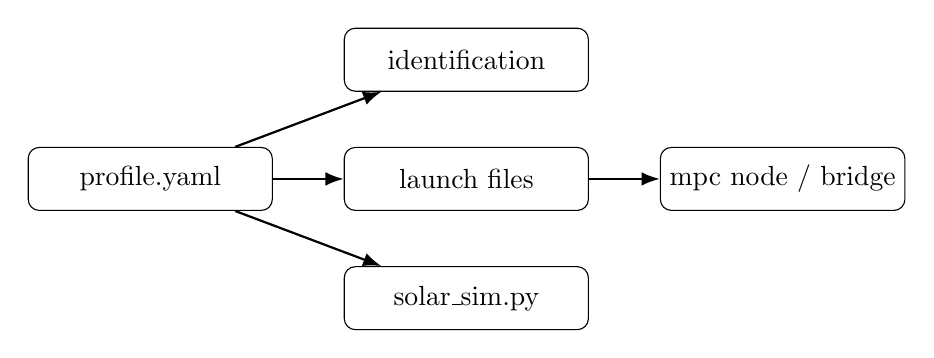
\begin{tikzpicture}[
  node distance=7mm and 9mm,
  box/.style={draw, rounded corners, align=center, minimum width=31mm, minimum height=8mm},
  arr/.style={-Latex, thick}
]
\node[box] (profile) {profile.yaml};
\node[box, right=of profile] (launch) {launch files};
\node[box, below right=of profile] (sim) {solar\_sim.py};
\node[box, above right=of profile] (identify) {identification};
\node[box, right=of launch] (live) {mpc node / bridge};
\draw[arr] (profile) -- (launch);
\draw[arr] (profile) -- (sim);
\draw[arr] (profile) -- (identify);
\draw[arr] (launch) -- (live);
\end{tikzpicture}
\end{center}

\subsection{既定 profile}
PowerShell の既定 path は \sourcepath{config/solar/bwsc_2027_demo.yaml} である。
これは \sourcepath{project_packages/bwsc2027_template/} を参照する wrapper profile であり、
空テンプレートを source 側から正しく叩けるようにするためのものである。
したがって、
\begin{itemize}[leftmargin=1.5em]
  \item build / forecast / identify の入口確認
  \item profile 構造確認
\end{itemize}
には使えるが、実走や full sim には、実データを入れた package profile を指定する必要がある。

\section{mode 別に何が起きるか}
\subsection{sim}
\begin{center}
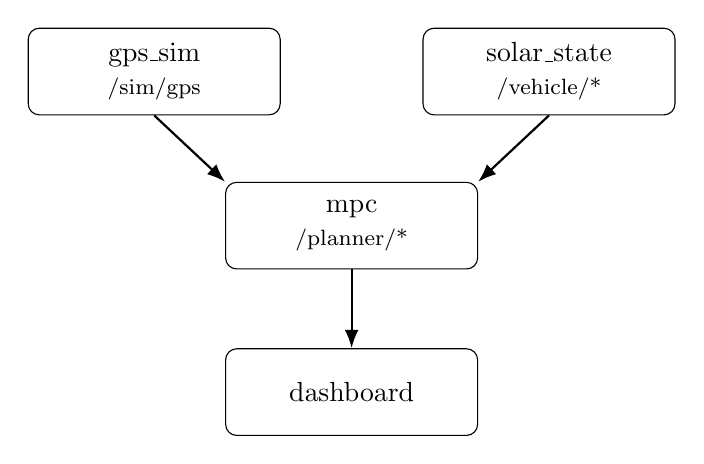
\begin{tikzpicture}[
  node distance=10mm and 18mm,
  box/.style={draw, rounded corners, align=center, minimum width=32mm, minimum height=11mm},
  arr/.style={-Latex, thick}
]
\node[box] (gps) {gps\_sim\\\footnotesize /sim/gps};
\node[box, right=of gps] (state) {solar\_state\\\footnotesize /vehicle/*};
\node[box, below=14mm of $(gps)!0.5!(state)$] (mpc) {mpc\\\footnotesize /planner/*};
\node[box, below=of mpc] (dash) {dashboard};
\draw[arr] (gps.south) -- (mpc.north west);
\draw[arr] (state.south) -- (mpc.north east);
\draw[arr] (mpc) -- (dash);
\end{tikzpicture}
\end{center}
planner speed command は次周期の gps/state 伝播へ戻る。図では線の交差を避けるため feedback 線を省略した。

offline detail CSVでは、\sourcepath{step\_dt\_sec} が下位指令周期で通常1秒である。
\sourcepath{outer\_step\_requested\_dt\_sec=600}に対して
\sourcepath{outer\_step\_actual\_dt\_sec}が11.747秒などになるのは、次の制御停止、
走行時間窓、天候格子、上位速度区間の境界で外側ステップを正確に分割するためである。
境界直前の\sourcepath{step\_dt\_sec}だけは1秒未満になり得るが、1 Hz指令の欠落ではない。

\begin{itemize}[leftmargin=1.5em]
  \item \sourcepath{gps_sim_node}: route waypoint 上を planner 指令速度で進め、\sourcepath{/sim/gps} を出す。
  \item \sourcepath{solar_state_node}: 同じ planner 指令速度から、\sourcepath{/vehicle/speed_kmh}, \sourcepath{/vehicle/s_km}, \sourcepath{/vehicle/batt_*}, \sourcepath{/vehicle/solar_power_w} を出す。
  \item \sourcepath{mpc_node}: profile の forecast / route / maps / model / mpc を読み、上位再計画と下位指令を出す。
  \item \sourcepath{dashboard_node}: 現在値と plan を 1 画面 API 化する。
\end{itemize}

\subsection{measure}
\begin{itemize}[leftmargin=1.5em]
  \item \sourcepath{distance_node}: \sourcepath{/vehicle/speed_kmh} を積分して \sourcepath{/vehicle/s_km} を出す。
  \item \sourcepath{grade_node}: GPS / altitude / distance から勾配を出す。
  \item \sourcepath{solar_logger_node}: 電池、PV、風、planner、校正値、WiFi 生文字列、system 状態を同一時刻行の CSV にする。
  \item \sourcepath{dashboard_node}: 計測中の値を可視化する。
\end{itemize}

\subsection{live}
\begin{itemize}[leftmargin=1.5em]
  \item \sourcepath{weather_fetch_node}: 現在の GPS または fallback 座標で Open-Meteo forecast を取得し、planner の読む CSV へ保存する。
  \item \sourcepath{mpc_node}: 1 時間再計画や 1 Hz lower command を行う本体。
  \item \sourcepath{solar_autocal_node}: 観測 solar / pack power と planner 予測の差から、\sourcepath{/calib/*} を publish する。
  \item \sourcepath{speed_command_bridge_node}: \sourcepath{/planner/speed_cmd} を安全な速度勾配に整形し、実車側の topic / UDP に渡す。
\end{itemize}
Open-Meteo archiveは経路上の日射計による独立観測ではなく、model/reanalysisである。
従って予報・欠測補間には使えるが、PV mapの高精度認証を単独では行わない。
no-trouble方策探索は、地点・時刻ごとのarchive瞬時GHI/DNI/DHIを保持する
\sourcepath{bwsc2025_nominal_fullcourse_weather_grid.csv}だけを使う。
\sourcepath{bwsc2025_historical_pv_conditioned_weather_grid.csv}は実車PVから
逆補正した循環的な診断専用品であり、方策順位付け、受入、live入力には使わない。
同定用にはBOM Himawari hourly exposureを
\sourcepath{scripts/import_bom_satellite_solar.py}で経路・時刻へ対応付ける。
BOMまたは経路上POA、同期MPPT状態が無い場合は
\sourcepath{high_precision_gate_pass=false}のままとする。詳細監査は
\sourcepath{outputs/reports/weather_power_timestep_audit/weather_power_timestep_audit.pdf}
に保存する。

\subsection{live\_wifi}
\begin{center}
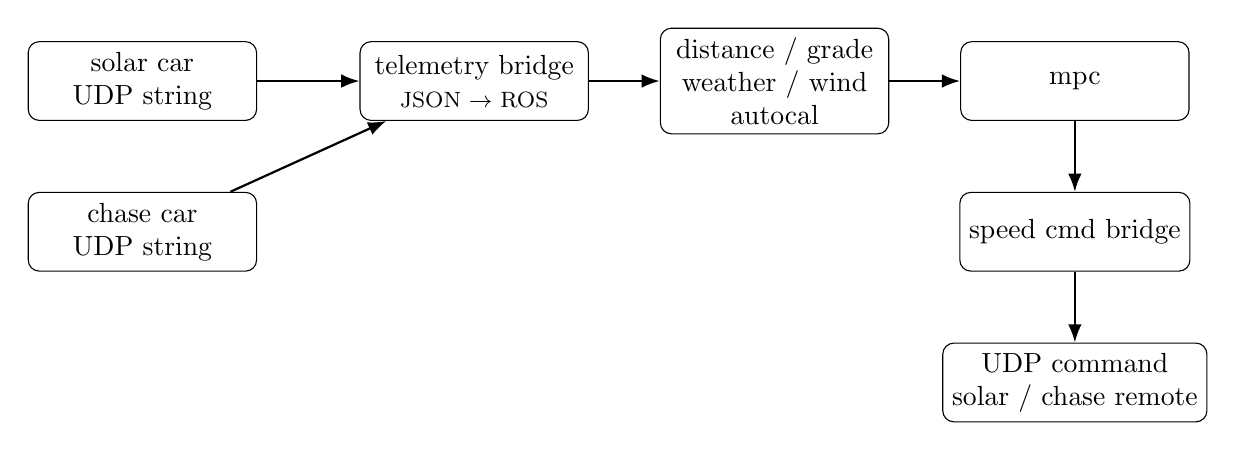
\begin{tikzpicture}[
  node distance=9mm and 9mm,
  box/.style={draw, rounded corners, align=center, minimum width=29mm, minimum height=10mm},
  arr/.style={-Latex, thick}
]
\node[box] (solar) {solar car\\UDP string};
\node[box, below=of solar] (chase) {chase car\\UDP string};
\node[box, right=13mm of solar] (tele) {telemetry bridge\\\footnotesize JSON $\rightarrow$ ROS};
\node[box, right=of tele] (est) {distance / grade\\weather / wind\\autocal};
\node[box, right=of est] (planner) {mpc};
\node[box, below=of planner] (cmd) {speed cmd bridge};
\node[box, below=of cmd] (remote) {UDP command\\solar / chase remote};
\draw[arr] (solar) -- (tele);
\draw[arr] (chase) -- (tele);
\draw[arr] (tele) -- (est);
\draw[arr] (est) -- (planner);
\draw[arr] (planner) -- (cmd);
\draw[arr] (cmd) -- (remote);
\end{tikzpicture}
\end{center}

\begin{itemize}[leftmargin=1.5em]
  \item \sourcepath{telemetry_text_bridge_node}: vehicle / chase からの JSON または key=value 文字列を受信し、ROS topic に展開する。
  \item \sourcepath{wind_correction_node}: 観測された向かい風から forecast CSV の \sourcepath{headwind_ms} を live 補正する。
  \item planner 側は修正済み forecast を見ながら upper/lower plan を更新する。
\end{itemize}

\subsection{launch file ごとの実起動 node}
以前は install 側にしか見えない source gap があったが、現在は launch / bridge / weather / profile utility を source 側へ戻してある。
したがって、チームは次の表だけで mode ごとの立ち上がりを追える。

\begin{center}
\begin{tabularx}{\linewidth}{>{\raggedright\arraybackslash}p{0.28\linewidth} >{\raggedright\arraybackslash}p{0.42\linewidth} X}
\toprule
launch file & 立ち上がる node & 用途 \\
\midrule
\sourcepath{launch/solarcar_sim.launch.py} &
\sourcepath{gps_sim_node}, \sourcepath{solar_state_node}, \sourcepath{mpc_node}, \sourcepath{dashboard_node} &
offline sim と上位/下位 plan の確認 \\
\sourcepath{launch/solar_measurement.launch.py} &
\sourcepath{solar_preflight_node}, \sourcepath{dashboard_node}, \sourcepath{solar_logger_node}, optional \sourcepath{distance_node}, optional \sourcepath{grade_node} &
実測収集と CSV 化 \\
\sourcepath{launch/solar_race_live.launch.py} &
\sourcepath{solar_preflight_node}, \sourcepath{mpc_node}, \sourcepath{dashboard_node}, \sourcepath{solar_logger_node}, \sourcepath{speed_command_bridge_node}, optional \sourcepath{distance_node}, \sourcepath{grade_node}, \sourcepath{weather_fetch_node}, \sourcepath{solar_autocal_node} &
通常 live 運用 \\
\sourcepath{launch/solar_race_live_wifi.launch.py} &
live node 一式 + \sourcepath{telemetry_text_bridge_node} + optional \sourcepath{wind_correction_node} &
WiFi 双方向運用 \\
\bottomrule
\end{tabularx}
\end{center}

\section{物理モデル}
\subsection{使っている基本式}
車速 $v$, 向かい風成分 $w$, 勾配角 $\theta$ に対する機械出力の近似は、
\[
  P_{\mathrm{mech}}
  = \left(
      \frac{1}{2}\rho C_dA (v+w)^2
      + m g C_{rr}\cos\theta
      + m g \sin\theta
    \right) v
\]
である。補機は駆動効率 map を通さず、電気側で直接加える。走行中と日中停車は
$P_{\mathrm{aux}}=P_{\mathrm{aux,stopped}}=21.021\,\mathrm{W}$、
日射が YAML の 20 W/m$^2$ 閾値以下となる夜間だけ
$P_{\mathrm{aux,night}}=0\,\mathrm{W}$ である。

なお、運用シミュレーション初期値
\sourcepath{simulation.soc0=0.98} と、履歴ログ再生だけに用いる潜在推定値
\sourcepath{identification.fitted_replay_soc0=0.966219} は別の状態である。
後者を前者へ書き戻してはならない。同定 writer は既定で両者を分離し、
回帰テストでもこの契約を固定している。

PV は、POA 日射 $G_{\mathrm{poa}}$、セル温度 $T_c$、パネル効率 map、MPPT 効率 map を用いて
\[
  P_{\mathrm{pv}} = \eta_{\mathrm{panel}}(G_{\mathrm{poa}}, T_c)\,
  \eta_{\mathrm{mppt}}(G_{\mathrm{poa}}, T_c)\,
  A_{\mathrm{pv}} G_{\mathrm{poa}}
\]
とする。

実車が WiFi で送る \sourcepath{solar_power_w} は、補正前の DC bus 実測値
$P_{\mathrm{solar,raw}}$ とする。日中停車かつ駆動電力がほぼゼロの標本だけを使い、
実測バッテリー電力との関係
\[
  P_{\mathrm{batt},i}
  =P_{\mathrm{aux}}-g_{\mathrm{solar}}P_{\mathrm{solar,raw},i}
  +\varepsilon_i
\]
から、外れ値に強い Huber M 推定
\[
  (\hat g_{\mathrm{solar}},\hat b)
  =\arg\min_{g,b}\sum_i
  \rho_{\delta}\!\left(
  P_{\mathrm{batt},i}-P_{\mathrm{aux}}
  +gP_{\mathrm{solar,raw},i}-b\right)
\]
を解く。$g$ は物理範囲内へ拘束し、切片 $b$、日別推定値の標準偏差、採用標本数も
同定 gate へ入れる。送信側は raw 値を送り、受信側が
$P_{\mathrm{solar}}=\hat g_{\mathrm{solar}}P_{\mathrm{solar,raw}}$ を一度だけ適用する。
送信側でも補正すると二重補正になるため禁止する。

パック出力は
\[
  P_{\mathrm{pack}} = P_{\mathrm{drive,dc}} - P_{\mathrm{regen,dc}}
  + P_{\mathrm{aux}} - P_{\mathrm{pv}}
\]
であり、SoC 更新は
\[
  z_{k+1} = z_k - \eta_{\mathrm{chg}}(I_k)
  \frac{I_k\Delta t_k}{3600Q_{\mathrm{nom}}}
\]
\[
  V_{p,k+1}=e^{-\Delta t/\tau_p}V_{p,k}
  +(1-e^{-\Delta t/\tau_p})R_pI_k,\qquad
  V_k=OCV(z_k)-I_kR_0-V_{p,k}
\]
である。

YATA の電池は 25 直列で、race-use 上限を $4.35\,\mathrm{V/cell}$ とするため、
\[
  V_{\max}=25\times4.35=108.75\,\mathrm{V}
\]
である。OCV map の最大値はこの上限以下でなければならず、profile の
\sourcepath{model.V\_max} は OCV map 最大値以上かつ $108.75\,\mathrm{V}$ に一致しなければ
ならない。OCV map がこの上限を超えたfitも不採用とする。この契約は静的監査と
回帰テストの双方で検査する。

現行MLE35候補のbattery-conditioned replayは、clean電力RMSE
$201.344\,\mathrm{W}$、clean電圧RMSE $0.968\,\mathrm{V}$ である。
天候・PV予測も含むend-to-end replayは、それぞれ
$246.088\,\mathrm{W}$、$2.113\,\mathrm{V}$、25 km energy RMSEは
$102.944\,\mathrm{Wh}$ である。battery-conditioned終端SoC誤差は
$0.006821$まで縮小したが、2831 km終端SoCの独立証拠は
0.332236から0.528667まで19.643 percentage points食い違う。
従って同期BMS coulomb count、rested OCV/温度、MPPT状態、POA日射が
揃うまで \sourcepath{high_precision_gate_pass=false} とする。終端一点の
一致だけをモデル高精度の証明にしてはならない。

旧4変数方策$[70,70,70,67]$ km/hはlegacy比較に限る。現行探索は
全3026.9 kmに対し、積分格子を5 km、1 km、0.1 kmへ細分し、速度制御間隔を
25 km、5 km、2 km、1 kmへ細分する。制御次元はfinish点を含めて
123、607、1515、3028である。4独立seed、8400世代、32,993,280候補を
CUDA CEMで提案し、各最終方策を別の1 Hz CPU simulatorで再計算する。
その後、固定方策の1/0.5/0.2/0.1 km積分格子と、独立最適化した
5/2/1 km制御方策の収束を判定する。CEMの最良値は連続領域全体の数学的な
大域最適性証明ではなく、exact replay、格子収束、車両model精度は別gateである。

向かい風成分は風速 $u$、風向 $\phi$、進行方位 $\psi$ から
\[
  w_{\mathrm{head}} = u \cos(\phi - \psi)
\]
で作る。

\subsection{実装でこれを使っている場所}
\begin{itemize}[leftmargin=1.5em]
  \item \sourcepath{mpc_solarcar/model.py}: 抵抗・PV・battery IV・SoC 更新
  \item \sourcepath{mpc_solarcar/mpc_node.py}: 上位 / 下位 MPC 評価
  \item \sourcepath{mpc_solarcar/upper_policy.py}: 受入済み速度方策の検証・補間と上位MPC初期解生成
  \item \sourcepath{scripts/solar_sim.py}: offline 全体 simulation
  \item \sourcepath{mpc_solarcar/solar_state_node.py}: sim 中の realtime 状態再生
\end{itemize}

\subsection{確認問題 2}
\begin{enumerate}[leftmargin=1.5em]
  \item SoC 更新の分母に入る nominal 容量は \fillin{$E_{\mathrm{nom}}$}{20mm} である。
  \item 向かい風成分は \fillin{$u\cos(\phi-\psi)$}{32mm} で与える。
\end{enumerate}

\section{実測ログからの MLE / fitting}
\subsection{pipeline}
\begin{center}
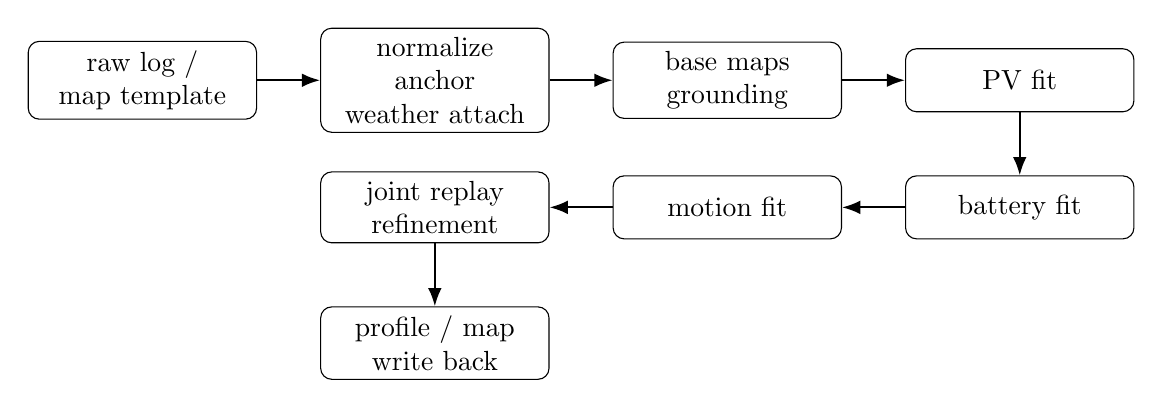
\begin{tikzpicture}[
  node distance=8mm and 8mm,
  box/.style={draw, rounded corners, align=center, minimum width=29mm, minimum height=8mm},
  arr/.style={-Latex, thick}
]
\node[box] (raw) {raw log /\\map template};
\node[box, right=of raw] (prep) {normalize\\anchor\\weather attach};
\node[box, right=of prep] (maps) {base maps\\grounding};
\node[box, right=of maps] (fit1) {PV fit};
\node[box, below=of fit1] (fit2) {battery fit};
\node[box, left=of fit2] (fit3) {motion fit};
\node[box, left=of fit3] (joint) {joint replay\\refinement};
\node[box, below=of joint] (write) {profile / map\\write back};
\draw[arr] (raw) -- (prep);
\draw[arr] (prep) -- (maps);
\draw[arr] (maps) -- (fit1);
\draw[arr] (fit1) -- (fit2);
\draw[arr] (fit2) -- (fit3);
\draw[arr] (fit3) -- (joint);
\draw[arr] (joint) -- (write);
\end{tikzpicture}
\end{center}

\subsection{軽量 pipeline}
\sourcepath{scripts/run_identification_pipeline.py} は、
\begin{itemize}[leftmargin=1.5em]
  \item \sourcepath{gps_track.csv}
  \item \sourcepath{battery_rest.csv}
  \item \sourcepath{battery_pulse.csv}
  \item \sourcepath{panel_sweep.csv}
  \item \sourcepath{drive_timeseries.csv}
\end{itemize}
から route / OCV / Rint / PV maps / vehicle scalar を構築する軽量 pipeline である。

\subsection{本 package の本格 replay fit}
\sourcepath{scripts/run_vehicle_identification.py} は、正規化済み replay log と既存 maps を使って、
\begin{align*}
  \mathcal{L}_{PV}(\theta_{PV})
  &= \sum_k \rho\!\left(P_{pv,k}^{obs} - P_{pv,k}^{pred}(\theta_{PV})\right), \\
  \mathcal{J}_{B}(\theta_B)
  &= \mathcal{L}_{B}(\theta_B) + \mathcal{R}_{B}(\theta_B), \\
  \mathcal{J}_{M}(\theta_M)
  &= \mathcal{L}_{M}(\theta_M) + \mathcal{R}_{M}(\theta_M),
\end{align*}
を順に最小化して PV, battery, motion を詰める。

ルート勾配は車両係数へ吸収せず、観測モデルとして別に検証する。DEM高度
$h(s)$ に Savitzky--Golay 平滑化を施した $\tilde h_{L}(s)$ から
\[
  q_{L,\delta}(s)=100\frac{d\tilde h_L(s+\delta)}{d(1000s)}
\]
を作り、平滑化長 $L$、距離オフセット $\delta$、仮の勾配倍率を
Day1--Day5 の電力RMSEで選ぶ。Day6を選択に使わず、同日のRMSEを悪化させない
候補だけを採択する。出力する
\sourcepath{adopted\_route\_profile.csv} は未スケールの $q_{L,\delta}$ を保持し、
$\gamma_{\mathrm{grade}}$ はその後のmotion fitで別に再同定する。summaryには候補数、
選択した $L,\delta$、train/holdout RMSEをすべて保存する。

ここで、
\begin{itemize}[leftmargin=1.5em]
  \item $\theta_{PV}$: panel gain, cell temperature gain
  \item $\theta_B$: $z_0, E_{\mathrm{nom}}, k_R, R_{\mathrm{line}}, \eta_{\mathrm{charge}}$
  \item $\theta_M$: $C_dA, C_{rr}, P_{\mathrm{aux}}, \gamma_{\mathrm{grade}}, k_{\eta}, k_w$
\end{itemize}
である。

\subsection{fit した値はどこへ入るか}
\begin{itemize}[leftmargin=1.5em]
  \item map そのもの: \sourcepath{profile.paths.*} が指す CSV
  \item scalar coefficient: \sourcepath{profile.model.*}
  \item planner weight / horizon: \sourcepath{profile.mpc.*}
  \item offline sim: \sourcepath{scripts/solar_sim.py} が profile から直読
  \item live: launch file が profile を展開し、\sourcepath{mpc_node} / bridge / weather node に渡す
\end{itemize}

\subsection{どのファイルを入れれば generic fitting が回るか}
\begin{center}
\begin{tabularx}{\linewidth}{>{\raggedright\arraybackslash}p{0.34\linewidth} X}
\toprule
template file & 役割 \\
\midrule
\sourcepath{templates/identification/observed_replay_log_template.csv} & 正規化 replay log の雛形 \\
\sourcepath{templates/identification/gps_track_template.csv} & route reconstruction の雛形 \\
\sourcepath{templates/identification/panel_sweep_template.csv} & panel / MPPT map \\
\sourcepath{templates/identification/battery_rest_template.csv} & OCV \\
\sourcepath{templates/identification/battery_pulse_template.csv} & Rint \\
\sourcepath{templates/identification/drive_timeseries_template.csv} & vehicle scalar fit \\
\sourcepath{templates/identification/source_map_catalog_template.csv} & 使用した元資料の整理 \\
\bottomrule
\end{tabularx}
\end{center}

\section{一画面 dashboard の読み方}
図\ref{fig:dashboard-demo}は、実際の \sourcepath{dashboard/} を教育用固定テレメトリで
1920$\times$1080描画したものである。全カードとsystem statusがスクロールなしで収まることを
目視確認した。固定値は \sourcepath{scripts/dashboard_demo_server.py} が返すため、実車値ではない。

\begin{figure}[htbp]
  \centering
  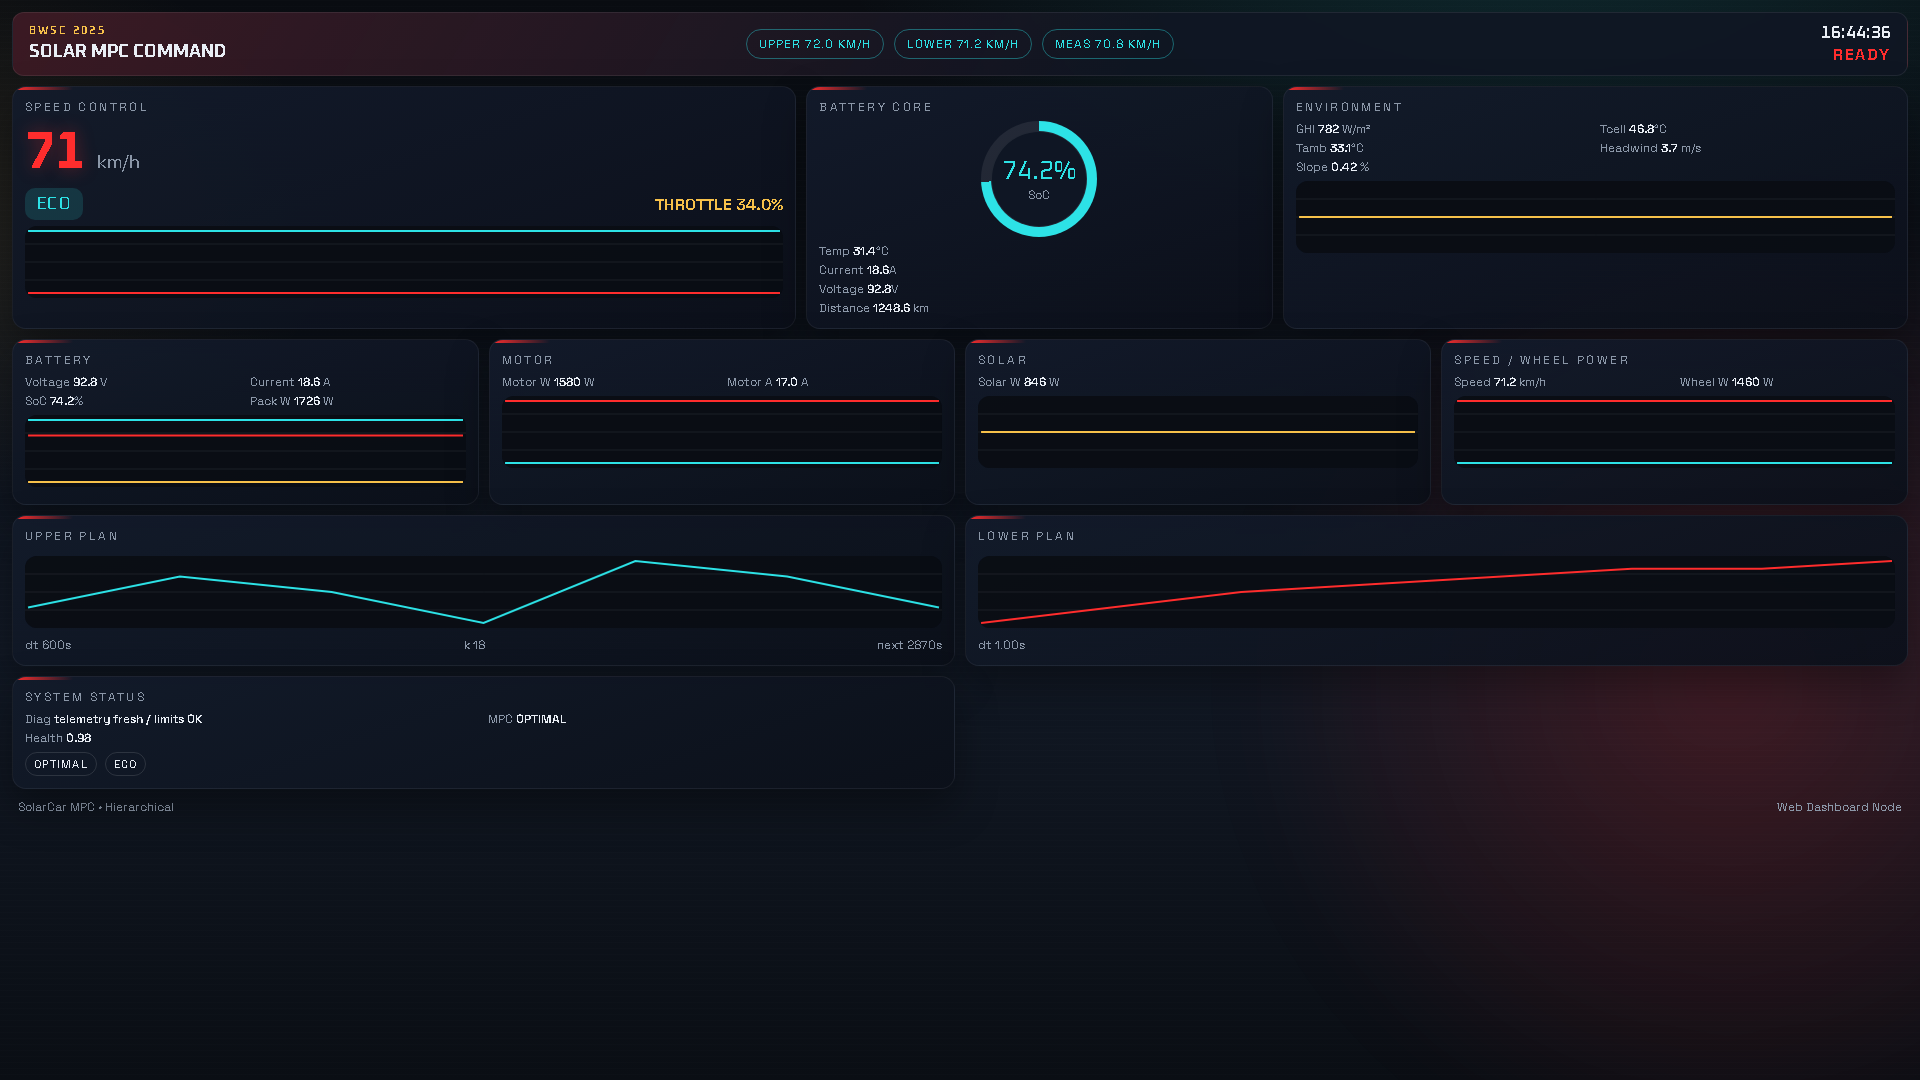
\includegraphics[width=\linewidth]{dashboard_demo_final.png}
  \caption{実dashboardの一画面デモ。上から現在指令、車両・環境、電力、上位・下位plan、健全性を並べる。}
  \label{fig:dashboard-demo}
\end{figure}

\begin{itemize}[leftmargin=1.5em]
  \item 上端の UPPER / LOWER / MEAS は、上位計画、1 Hz下位指令、実測速度である。差が継続すれば追従異常を疑う。
  \item SPEED CONTROL は最終速度指令、drive mode、throttle相当量を示す。実機へ送る値はrate limit後の値である。
  \item BATTERY CORE と BATTERY は SoC、温度、電圧、電流、pack電力、距離を示す。SoCだけでなく電圧・電流制約を同時に見る。
  \item ENVIRONMENT はPOA日射、セル・外気温、補正向かい風、勾配であり、上位予測の主要外乱である。
  \item MOTOR / SOLAR / SPEED-WHEEL POWER は、駆動、発電、車輪機械出力を分け、符号・効率mapの異常を切り分ける。
  \item UPPER PLAN は残距離の速度計画、LOWER PLAN は直近数秒の追従計画である。両者の時間尺度を混同しない。
  \item SYSTEM STATUS は telemetry freshness、limit、MPC solve状態、healthを示す。READYでもdiagを必ず読む。
\end{itemize}

教育用画面は repository root で
\begin{verbatim}
python scripts/dashboard_demo_server.py --port 18080
\end{verbatim}
を実行し、\sourcepath{http://127.0.0.1:18080}を開く。実運用ではこのデモを起動せず、
\sourcepath{dashboard_node.py} の \sourcepath{/api/state} を使用する。

\section{live\_wifi の送受信仕様}
\subsection{推奨方式}
推奨は UTF-8 の UDP JSON である。newline は不要、1 パケット 1 JSON を基本とする。
全 Raspberry Pi は起動前に NTP / chrony で UTC 同期する。
既定では \sourcepath{timestamp\_utc} または \sourcepath{ts\_unix} が必須であり、
5 秒より古い packet、2 秒より未来の packet、重複・時刻逆転 packet は
filter や ROS topic 更新の前に破棄される。

\subsection{ソーラーカー側から送る推奨 JSON}
\begin{verbatim}
{
  "type": "vehicle_state",
  "ts_unix": 1762500000.0,
  "speed_kmh": 72.3,
  "soc": 0.83,
  "batt_temp_c": 34.2,
  "batt_current_a": 8.5,
  "batt_voltage_v": 97.6,
  "solar_power_w": 410.0,
  "lat": -19.13542,
  "lon": 146.81235,
  "alt_m": 18.4,
  "wind_speed_ms": 6.8,
  "wind_dir_deg": 118.0,
  "course_deg": 176.5
}
\end{verbatim}

\subsection{伴走車側から送る推奨 JSON}
\begin{verbatim}
{
  "type": "chase_state",
  "ts_unix": 1762500001.0,
  "speed_kmh": 74.0,
  "lat": -19.13580,
  "lon": 146.81210,
  "alt_m": 18.1,
  "wind_speed_ms": 6.5,
  "wind_dir_deg": 121.0,
  "course_deg": 176.0
}
\end{verbatim}

\subsection{planner 側から返す JSON}
\begin{verbatim}
{
  "type": "planner_command",
  "ts_unix": 1762500002.0,
  "timestamp_utc": "2025-11-07T10:00:02Z",
  "planner": {
    "speed_cmd_kmh": 68.0,
    "upper_speed_cmd_kmh": 69.0,
    "drive_mode": "eco"
  },
  "vehicle": {
    "speed_kmh": 67.4,
    "soc": 0.81,
    "s_km": 412.3
  }
}
\end{verbatim}

\subsection{key=value fallback}
\sourcepath{telemetry_text_bridge_node.py} は JSON だけでなく
\begin{verbatim}
type=vehicle_state,speed_kmh=71.8,soc=0.82,batt_voltage_v=97.4
\end{verbatim}
のような key=value も構文として扱えるが、通常運用では同じ列に
\sourcepath{timestamp\_utc=...Z} または \sourcepath{ts\_unix=...} を必ず付ける。

\subsection{マイコン側の実装条件}
\begin{itemize}[leftmargin=1.5em]
  \item WiFi: 同一 LAN, UDP
  \item 文字コード: UTF-8
  \item 推奨周期: 1 Hz
  \item 起動前に NTP / chrony 同期を確認し、送信 packet に毎回 UTC 時刻を入れる
  \item パケット喪失を考え、planner command は 3 秒 timeout で無効化
  \item 受信未更新時はマイコン側でも fail-safe を持つ
  \item 参考: \sourcepath{scripts/wifi_vehicle_sender_example.py}
  \item 参考: \sourcepath{scripts/wifi_chase_sender_example.py}
  \item 参考: \sourcepath{templates/network/esp32_planner_receiver_example.ino}
\end{itemize}

\section{現在の maps / coefficients 研究候補例}
現時点で追跡しやすい fitted 研究候補は次の package である。
\par\smallskip
\sourcepath{project_packages/bwsc2025_fitted_mle19_energywindow_inertia/}
\par\smallskip
ここで示すMLE35はimmutableな未昇格研究候補であり、canonical live profileではない。
本番用\sourcepath{profile_operational_fine.yaml}は
$C_dA=0.109802$、$C_{rr}=0.006560$、
$P_{\mathrm{aux}}=P_{\mathrm{aux,stopped}}=20.891\,\mathrm{W}$、
$P_{\mathrm{aux,night}}=0\,\mathrm{W}$、
$E_{\mathrm{nom}}=2899.987\,\mathrm{Wh}$、$Q_{\mathrm{nom}}=31.783316\,\mathrm{Ah}$
を保持している。旧値の方が正確という意味ではなく、独立モデル検証ゲートを通らない研究候補を
本番へ混入させないための分離である。

このMLE35候補の\sourcepath{current_maps_and_coefficients.md}要約を参照すると、
候補内で評価するassetは次である。

\begin{center}
\begin{tabularx}{\linewidth}{>{\raggedright\arraybackslash}p{0.34\linewidth} X}
\toprule
asset & 役割 \\
\midrule
\sourcepath{outputs/identification/runs/mle35_expanded_grade_single_source_ultra_v1/adopted_maps/drive_eff_map.csv} と eco/power 派生 & 駆動効率 map \\
\sourcepath{outputs/identification/runs/mle35_expanded_grade_single_source_ultra_v1/adopted_maps/regen_eff_map.csv} と eco/power 派生 & 回生効率 map \\
\sourcepath{outputs/identification/runs/mle35_expanded_grade_single_source_ultra_v1/adopted_maps/Rint_T_by_soc_fitted_grounded.csv} & 温度・SoC 依存内部抵抗 map \\
\sourcepath{outputs/identification/runs/mle35_expanded_grade_single_source_ultra_v1/adopted_maps/panel_eff_map.csv} & パネル効率 map \\
\sourcepath{outputs/identification/runs/mle35_expanded_grade_single_source_ultra_v1/adopted_maps/mppt_eff_map.csv} & MPPT 効率 map \\
\sourcepath{outputs/identification/runs/mle35_expanded_grade_single_source_ultra_v1/adopted_maps/ocv_soc_curve.csv} & OCV-SoC 曲線 \\
\sourcepath{data/weather/bwsc2025_nominal_fullcourse_weather_grid.csv} & 大会全体 nominal weather grid \\
\sourcepath{data/observed/bwsc2025_observed_log_5s.csv} & progress reference / replay log \\
\bottomrule
\end{tabularx}
\end{center}

同要約に出ている代表 scalar は、
\[
  m = 235.0,\quad
  C_dA = 0.111167,\quad
  C_{rr} = 0.006262,\quad
  P_{\mathrm{aux}} = 21.021\,\mathrm{W},
\]
\begin{align*}
  P_{\mathrm{aux,stopped}} &= 21.021\,\mathrm{W}, &
  P_{\mathrm{aux,night}} &= 0\,\mathrm{W},\\
  E_{\mathrm{nom}} &= 3011.000\,\mathrm{Wh}, &
  Q_{\mathrm{nom}} &= 33.000\,\mathrm{Ah},\\
  R_p &= 0.084252\,\Omega, &
  \tau_p &= 73.595\,\mathrm{s},\\
  \mathrm{panel\_gain} &= 0.712687, &
  \mathrm{drive\_eff\_scale} &= 1.034296,\\
  \mathrm{solar\_measurement\_gain} &= 0.922613, &
  \mathrm{rint\_scale} &= 0.900000.
\end{align*}
である。

no-trouble方策評価はトラブル停車を除くが、公式control stopを除かない。
\sourcepath{data/race/bwsc2025_official_control_stops.yaml}に9地点、各1800秒、
公式開閉時刻、Adelaide締切\sourcepath{2025-08-29T08:00:00Z}を保存する。
早着時は開場まで待機し、control stop閉鎖後またはfinish締切後の到着は、
CUDA surrogateと厳密1 Hz replayの両方で不成立とする。時刻根拠は
\url{https://assets.worldsolarchallenge.org/app/uploads/2025/08/20102713/BWSC-2025-Official-Program-v4.pdf}
のcontrol-stop表である。17:30にはCruiser Class最終到着との脚注があるため、
報告書ではこの注記も保持する。

\section{実際の使い方}
\subsection{template package を育てる流れ}
\begin{enumerate}[leftmargin=1.5em]
  \item \sourcepath{project_packages/bwsc2027_template/} に route, weather, map, schedule, identification raw を入れる。
  \item \cmd{python scripts/run\_identification\_pipeline.py --profile\_yaml <profile>} で軽量 map 作成を行う。
  \item replay log があるなら \cmd{python scripts/run\_vehicle\_identification.py --profile <profile>} で本格 fit を行う。
  \item
  \begin{tabular}[t]{@{}l@{}}
  \ttfamily powershell -ExecutionPolicy Bypass -File .\textbackslash SolarSim.ps1 \\
  \ttfamily \ \ -Action simulate -Profile <profile>
  \end{tabular}
  で full sim を確認する。
  \item
  \begin{tabular}[t]{@{}l@{}}
  \ttfamily powershell -ExecutionPolicy Bypass -File .\textbackslash SolarSim.ps1 \\
  \ttfamily \ \ -Mode live\_wifi -Action up -Profile <profile>
  \end{tabular}
  で実運用へ入る。
\end{enumerate}

\subsection{典型コマンド}
\begin{verbatim}
powershell -ExecutionPolicy Bypass -File .\SolarSim.ps1 -Action build
powershell -ExecutionPolicy Bypass -File .\SolarSim.ps1 -Action forecast
powershell -ExecutionPolicy Bypass -File .\SolarSim.ps1 -Action simulate `
  -Profile <profile>
powershell -ExecutionPolicy Bypass -File .\SolarSim.ps1 -Mode live_wifi -Action up `
  -Profile <profile>
python scripts/run_vehicle_identification.py --profile <profile>
\end{verbatim}

\subsection{Slurmでの多忠実度探索と独立受入}
GPU CEMは多数方策を提案し、CPU側は固定方策1 Hz再計算と格子収束だけを受入根拠にする。
GPU探索は1割当内で4 seedを直列化する。
環境変数\sourcepath{REPLICATE_INDEX=0..3}を別jobへ与えた場合だけ、schedulerが
GPU quotaの範囲で並列化する。1 GPU内へ4 CUDA processを競合配置せず、
受入側のCPU処理には後述の最大12並列を用いる。
\begin{verbatim}
sbatch --export=ALL,SOLAR_GPU_ROOT=$PWD,\
PYTHON_BIN=$HOME/.venvs/mpc_gpu/bin/python \
  scripts/run_solar_gpu_concurrent_campaign.sbatch <profile> <campaign_dir>

sbatch --dependency=afterok:<job_id> --export=ALL,SOLAR_GPU_ROOT=$PWD,\
PYTHON_BIN=$HOME/.venvs/mpc_gpu/bin/python \
  scripts/run_solar_gpu_acceptance_pipeline.sbatch \
  <profile> <campaign_dir> <acceptance_dir>
\end{verbatim}
独立ジョブ方式では\sourcepath{campaign_submission.yaml}の
\sourcepath{finalize_job_id}を次の依存指定に使う。
\begin{verbatim}
sbatch --dependency=afterok:<finalize_job_id> ...
\end{verbatim}
finalizerは4本すべての\sourcepath{control_1km/latest_policy.csv}を
確認してから\sourcepath{CAMPAIGN_COMPLETE}を書く。
また、投入時に profile の SHA-256 を \sourcepath{campaign_submission.yaml}へ保存し、
coarse、fine、ultra、control-refine、finalize の全 stage が開始前に同じ hash を
再計算する。探索中に YAML が変更された場合は、その stage を失敗させる。
これにより異なる車両モデルの評価値を同じ収束履歴へ混在させない。

受入ジョブは5、2、1 kmの3格子を並列実行し、各格子内の4 seedも並列実行する。
従って要求した16 CPUのうち最大12 CPUを用いて、固定policyの100 m予測と1 Hz全行程再生を行う。
各seedは固有のprofile、manifest、detail CSV、判定表を持ち、全worker終了後にだけ
最速の可行seedを選択する。1 seedの未可行は候補棄却であり、出力欠損または
全seed未可行の場合だけそのstageを失敗とする。

単一GPU割当方式では4本の\sourcepath{PIPELINE_COMPLETE}、独立ジョブ方式では
4本の最終policy、さらに\sourcepath{CAMPAIGN_COMPLETE}、
\sourcepath{ACCEPTANCE_COMPLETE}を確認する。exact候補が無い、または格子収束が
未達なら\sourcepath{ACCEPTANCE_FAILED}となり、live profileへ昇格してはならない。
exact 1 Hz replayとmesh収束だけが通った段階では
\sourcepath{POLICY_ACCEPTANCE_COMPLETE}と
\sourcepath{profile_exact_selected_research.yaml}だけを作る。独立車両model gateも
通った場合に限り\sourcepath{ACCEPTANCE_COMPLETE}、
\sourcepath{profile_exact_selected.yaml}、
\sourcepath{profile_live_mpc_learned.yaml}を作る。従って
\sourcepath{POLICY_ACCEPTANCE_COMPLETE}と\sourcepath{ACCEPTANCE_FAILED}の併存は、
方策計算は合格したが車両modelを実運用認定できないことを表す。
制御格子は5 km、2 km、1 kmで独立に最適化したpolicyを使う。最細分の
\sourcepath{--policy}は必ず1 kmへ割り当て、2 km policyを上書きしない。
受入成功時は二つのprofileを生成する。\sourcepath{profile_exact_selected.yaml}は
方策を固定した1 Hz再現試験専用である。\sourcepath{profile_live_mpc_learned.yaml}は
同じCSVを\sourcepath{paths.initial_upper_policy_csv}へ設定するが固定しない。
\sourcepath{mpc_node.py}は起動時にこの方策を現在の制御格子へ補間し、上位MPCの
初期解としてだけ使用する。その後は実測SoC、現在距離、更新予報、制約を使って
上位問題を再度解き、次回からは直前のMPC解を移動後の格子へ補間する。従って
GPU CEMはoffline proposer、live指令の最終決定権はreceding-horizon MPCにある。
全成果物の日本語TeX/PDFは次で作る。
\begin{verbatim}
python scripts/generate_gpu_acceptance_report.py \
  --profile <profile> --campaign-dir <campaign_dir> \
  --acceptance-dir <acceptance_dir> --fit-summary <fit_summary> \
  --promotion-gate <promotion_gate.json> --output-dir <report_dir>
\end{verbatim}
この報告書はGPU収束履歴、全exact順位、1 Hz fullsim、積分・制御格子収束、
独立モデルgateを統合する。

\subsection{ソーラーカー専用クリーン copy の作成}
\begin{itemize}[leftmargin=1.5em]
  \item
  \begin{tabular}[t]{@{}l@{}}
  \ttfamily python scripts/create\_solarcar\_only\_package.py \\
  \ttfamily \ \ --output\_dir exports/solarcar\_only\_package\_20260712
  \end{tabular}
  を実行すると、配布用の整理済み copy を生成する。
  \item copy 側では \sourcepath{passo_*} launch、\sourcepath{passo_run.sh}、磁力関連 source / script、旧 \sourcepath{bwsc2025_fitted_mle*} package、build / install / log / outputs を含めない。
  \item さらに copy 内の \sourcepath{setup.py} から磁力 entry point を除去し、\sourcepath{mpc\_node.py} は solar 専用初期化に固定する。
  \item 配布相手には、この clean copy と \sourcepath{docs/solar_all_in_one_manual/solar_all_in_one_manual.pdf} をそのまま渡せばよい。
\end{itemize}

\subsection{確認問題 3}
\begin{enumerate}[leftmargin=1.5em]
  \item 軽量 map 作成の入口は \fillin{\sourcepath{scripts/run_identification_pipeline.py}}{48mm} である。
  \item full-race offline sim の入口は \fillin{\sourcepath{scripts/solar_sim.py}}{38mm} である。
  \item live で Open-Meteo を取りに行く node は \fillin{\sourcepath{weather_fetch_node}}{34mm} である。
\end{enumerate}

\section{まとめ}
\begin{itemize}[leftmargin=1.5em]
  \item 入口は \sourcepath{SolarSim.ps1} $\rightarrow$ \sourcepath{scripts/solar_control.sh} である。
  \item mode ごとの launch と node は source 側で追える状態へ戻した。
  \item profile は sim / live / identify の唯一の接着剤であり、maps と scalar の反映先でもある。
  \item MLE / replay fit は、PV, battery, motion, joint replay を順に詰め、その結果を profile と maps に書き戻す。
  \item live\_wifi では、JSON 文字列テレメトリ $\rightarrow$ ROS topic $\rightarrow$ weather / wind / autocal $\rightarrow$ MPC $\rightarrow$ speed command bridge という一直線の流れで理解するのが最も見通しが良い。
\end{itemize}

\end{document}
